\documentclass[11pt,a4paper]{article}

\usepackage{geometry}
\geometry{legalpaper, margin=1in}

\usepackage[utf8]{inputenc}
\usepackage[T1]{fontenc}
\usepackage{amsmath,amssymb,amsfonts}
\usepackage{graphicx}
\usepackage{float}
\usepackage{hyperref}
\usepackage{xcolor}
\usepackage{caption}
\usepackage{subcaption}
\usepackage{amsmath, amssymb}
\usepackage{graphicx}
\usepackage{booktabs}


\title{Methods in Computational Neuroscience\\
[Your Project Title]}
\author{Sepehr Saeedpour}
\date{June 2025}

\begin{document}

\maketitle

\section*{Introduction}
Ring attractor networks provide a foundational computational framework for representing circular, continuous variables such as head direction, spatial orientation, or phase information by sustaining a localized "bump" of persistent neural activity. These activity bumps can stably occupy any position along a one-dimensional ring manifold, forming a continuum of marginally stable fixed points. This property emerges from a "Mexican-hat" connectivity profile characterized by sharp local excitation balanced against broader inhibition, effectively flattening the network's energy landscape. As a result, even infinitesimal velocity inputs can smoothly shift the bump without drift.

Classical theoretical analyses, developed for networks in the large-N limit, predict that an ideally flat manifold, and thus near-perfect precision, requires large neuron counts. With fewer neurons, this ring manifold was traditionally expected to fragment into discrete attractor states, causing the emergence of preferred orientations, spontaneous drift, and velocity integration thresholds. Consequently, classical theory suggests a direct trade-off between network size and discretization errors, implying biological circuits must be large to achieve accurate continuous dynamics.

Recent electron microscopy reconstructions of compass neurons in Drosophila melanogaster challenge this perspective. These studies have shown that the fly's head-direction system comprises remarkably few computational units, far fewer than classical models would suggest necessary. Complementary two-photon calcium imaging further reveals that this minimal network can nonetheless maintain a smoothly rotating activity bump that accurately tracks the fly’s head direction in darkness, exhibiting negligible drift and no clear discretized orientations. These empirical findings demonstrate that biologically accurate continuous attractors can be achieved with surprising neuronal economy.

Inspired by these results, Noorman et al. (2024) constructed a threshold-linear ring attractor model with just six neurons. They analytically demonstrated that by fine-tuning local excitation to one of several discrete "sweet-spot" values, the curvature of the network’s energy landscape can be reduced to zero. This effectively creates a seamless ring composed of multiple interconnected line attractors, resulting in marginally stable states. Numerical simulations confirmed that these networks could sustain drift-free persistent activity and perform linear integration of velocity inputs, even at arbitrarily small magnitudes.

However, achieving such performance in small networks requires precise tuning, introducing inherent fragility. Analytical bounds and numerical experiments indicate that the parameter ranges supporting flat landscapes narrow as the network size decreases, with both sensitivity to mistuning and susceptibility to noise increasing roughly linearly as networks shrink. Nonetheless, the existence of highly functional yet minimal neural architectures, as exemplified by the fly compass, implies that continuous-variable computations may be more computationally economical and widespread than previously thought. These findings also provide valuable design principles for compact artificial navigation systems inspired by insect brains.


\section*{Methods}
\subsection{Mathematical Framework}
The dynamics of neuron \( j \) in a velocity-driven ring attractor network are governed by:

\begin{equation}
\tau \frac{d h_j}{dt} = -h_j + \frac{1}{N} \sum_{k=1}^N \left( W^{\text{sym}}_{jk} + v_{\text{in}} W^{\text{asym}}_{jk} \right) \phi(h_k) + c_{\text{ff}},
\label{eq:ring_dynamics}
\end{equation}

where \(\phi(h)\) represents the threshold-linear activation function:
\[
\phi(h) = [h]_+ = \max(0, h).
\]

The network's connectivity structure consists of symmetric and asymmetric components:
\begin{align}
W^{\text{sym}}_{jk} &= J_I + J_E \cos(\theta_j - \theta_k), \\
W^{\text{asym}}_{jk} &= \sin(\theta_j - \theta_k).
\end{align}

The symmetric component combines uniform inhibition (\(J_I\)) with local excitation modulated by the neurons' preferred orientations, while the asymmetric component enables directional sensitivity and velocity integration. Tables 1 and 2 detail the functional roles of all parameters in this framework.

% where $\theta_i = 2\pi i/N$ represents the preferred direction of neuron $i$, $J_E$ and $J_I$ control excitatory and inhibitory coupling strengths, $J_{vel}$ determines velocity integration strength, and $\delta$ introduces phase shifts for directional selectivity.

\begin{table}[h!]
\centering
\begin{tabular}{@{}llp{9cm}@{}}
\toprule
\textbf{Symbol} & \textbf{Type} & \textbf{Description} \\
\midrule
\( h_j \) & variable & Total synaptic input (current) to neuron \( j \) \\
\( \phi(h) \) & function & Threshold-linear activation function: \( \phi(h) = \max(0, h) \) \\
\( \tau \) & parameter & Neural integration time constant (slower when large) \\
\( N \) & parameter & Total number of neurons arranged on a ring \\
\( \theta_j \) & parameter & Preferred orientation of neuron \( j \), uniformly distributed in \([0, 2\pi)\) \\
\( v_{\text{in}} \) & input & External angular velocity input to the network \\
\( c_{\text{ff}} \) & parameter & Constant feedforward bias input to all neurons \\
\( J_E \) & parameter & Strength of the \emph{tuned} (cosine) component of connectivity (local excitation) \\
\( J_I \) & parameter & Strength of the \emph{untuned} (uniform) component of connectivity (global inhibition) \\
% \( W^{\text{sym}}_{jk} \) & derived & Symmetric connectivity: \( J_I + J_E \cos(\theta_j - \theta_k) \) \\
% \( W^{\text{asym}}_{jk} \) & derived & Asymmetric (velocity-sensitive) connectivity: \( \sin(\theta_j - \theta_k) \) \\
\bottomrule
\end{tabular}
\caption{Variables and parameters used in Eq. 1 and the network structure.}
\end{table}


\begin{table}[h!]
\centering
\begin{tabular}{@{}lp{12cm}@{}}
\toprule
\textbf{Parameter} & \textbf{Effect on Network Dynamics} \\
\midrule
\( \tau \) & Governs the timescale of neural responses. Large \( \tau \): slower integration, more smoothing. Small \( \tau \): rapid but potentially unstable dynamics. \\
\( J_E \) & Controls the strength of local excitation. Must be sufficiently strong to generate a stable bump. Too low: no bump. Too high: narrow or unstable bump. \\
\( J_I \) & Controls global inhibition. Helps normalize activity across neurons, limits bump width, prevents runaway excitation. \\
\( v_{\text{in}} \) & Angular velocity input that biases bump motion. Positive or negative values move the bump CW or CCW around the ring. \\
\( c_{\text{ff}} \) & Background excitation to ensure enough baseline input. Influences overall bump amplitude and whether any neurons are active. \\
\bottomrule
\end{tabular}
\caption{Qualitative effects of key parameters on bump dynamics and attractor behavior.}
\end{table}

\subsection{Simulation and Example Network}

\subsubsection*{Simulation Procedure}

To investigate the attractor landscape of the ring network, we simulated its dynamics across a range of initial conditions and network parameters. For each parameter setting, the network’s architecture was defined by a symmetric weight matrix implementing local excitation and global inhibition, and an antisymmetric matrix representing velocity-modulated input. To probe the full range of attractor states, we initialized the network with 1000 distinct activity patterns, each corresponding to a cosine-shaped “bump” of activity centered at a different orientation $\psi$ around the ring. Each initial state was constructed using the analytical bump formula from Eq. (S16) in the Supplementary Information:

\begin{equation}
h_j^{(0)} = a \left[\cos(\theta_j - \psi) - \cos\left(\frac{w}{2}\right)\right]_+
\end{equation}


where $\theta_j = \frac{2\pi(j-1)}{N}$ is the preferred orientation of neuron $j$, $a$ is the bump amplitude, and $w$ is the bump width. This ensures the bump is centered at $\psi$ and spans a localized region on the ring.

The network dynamics were simulated over a time interval $T = 3\,\text{s}$ using the Euler method with a fixed time step of $\Delta t = 0.01\,\text{s}$. For each initial condition, the system was numerically integrated until convergence to a fixed point. The resulting final activity vectors were recorded and collectively represent the attractor states of the network under the specified parameters.

\subsubsection*{Example Network}

We visualize the network connectivity and bump dynamics for a ring attractor model with $N = 6$ neurons, using parameters $J_E = 3.0$, $J_I = -1.0$, and $\tau = 0.1$. The symmetric connectivity matrix $W^{\text{sym}}$ defines local excitation and broad inhibition via a cosine profile, while the asymmetric matrix $W^{\text{asym}}$ supports velocity-driven shifts in bump position. After simulating the network dynamics from a cosine-shaped initial condition, the system evolves to a stable bump of activity. The support of this bump identifies a subset of active neurons, whose interactions define a principal submatrix of $W^{\text{sym}}$. This submatrix governs the local linear dynamics and plays a key role in determining the stability of the attractor.

\begin{figure}[htbp]
    \centering
    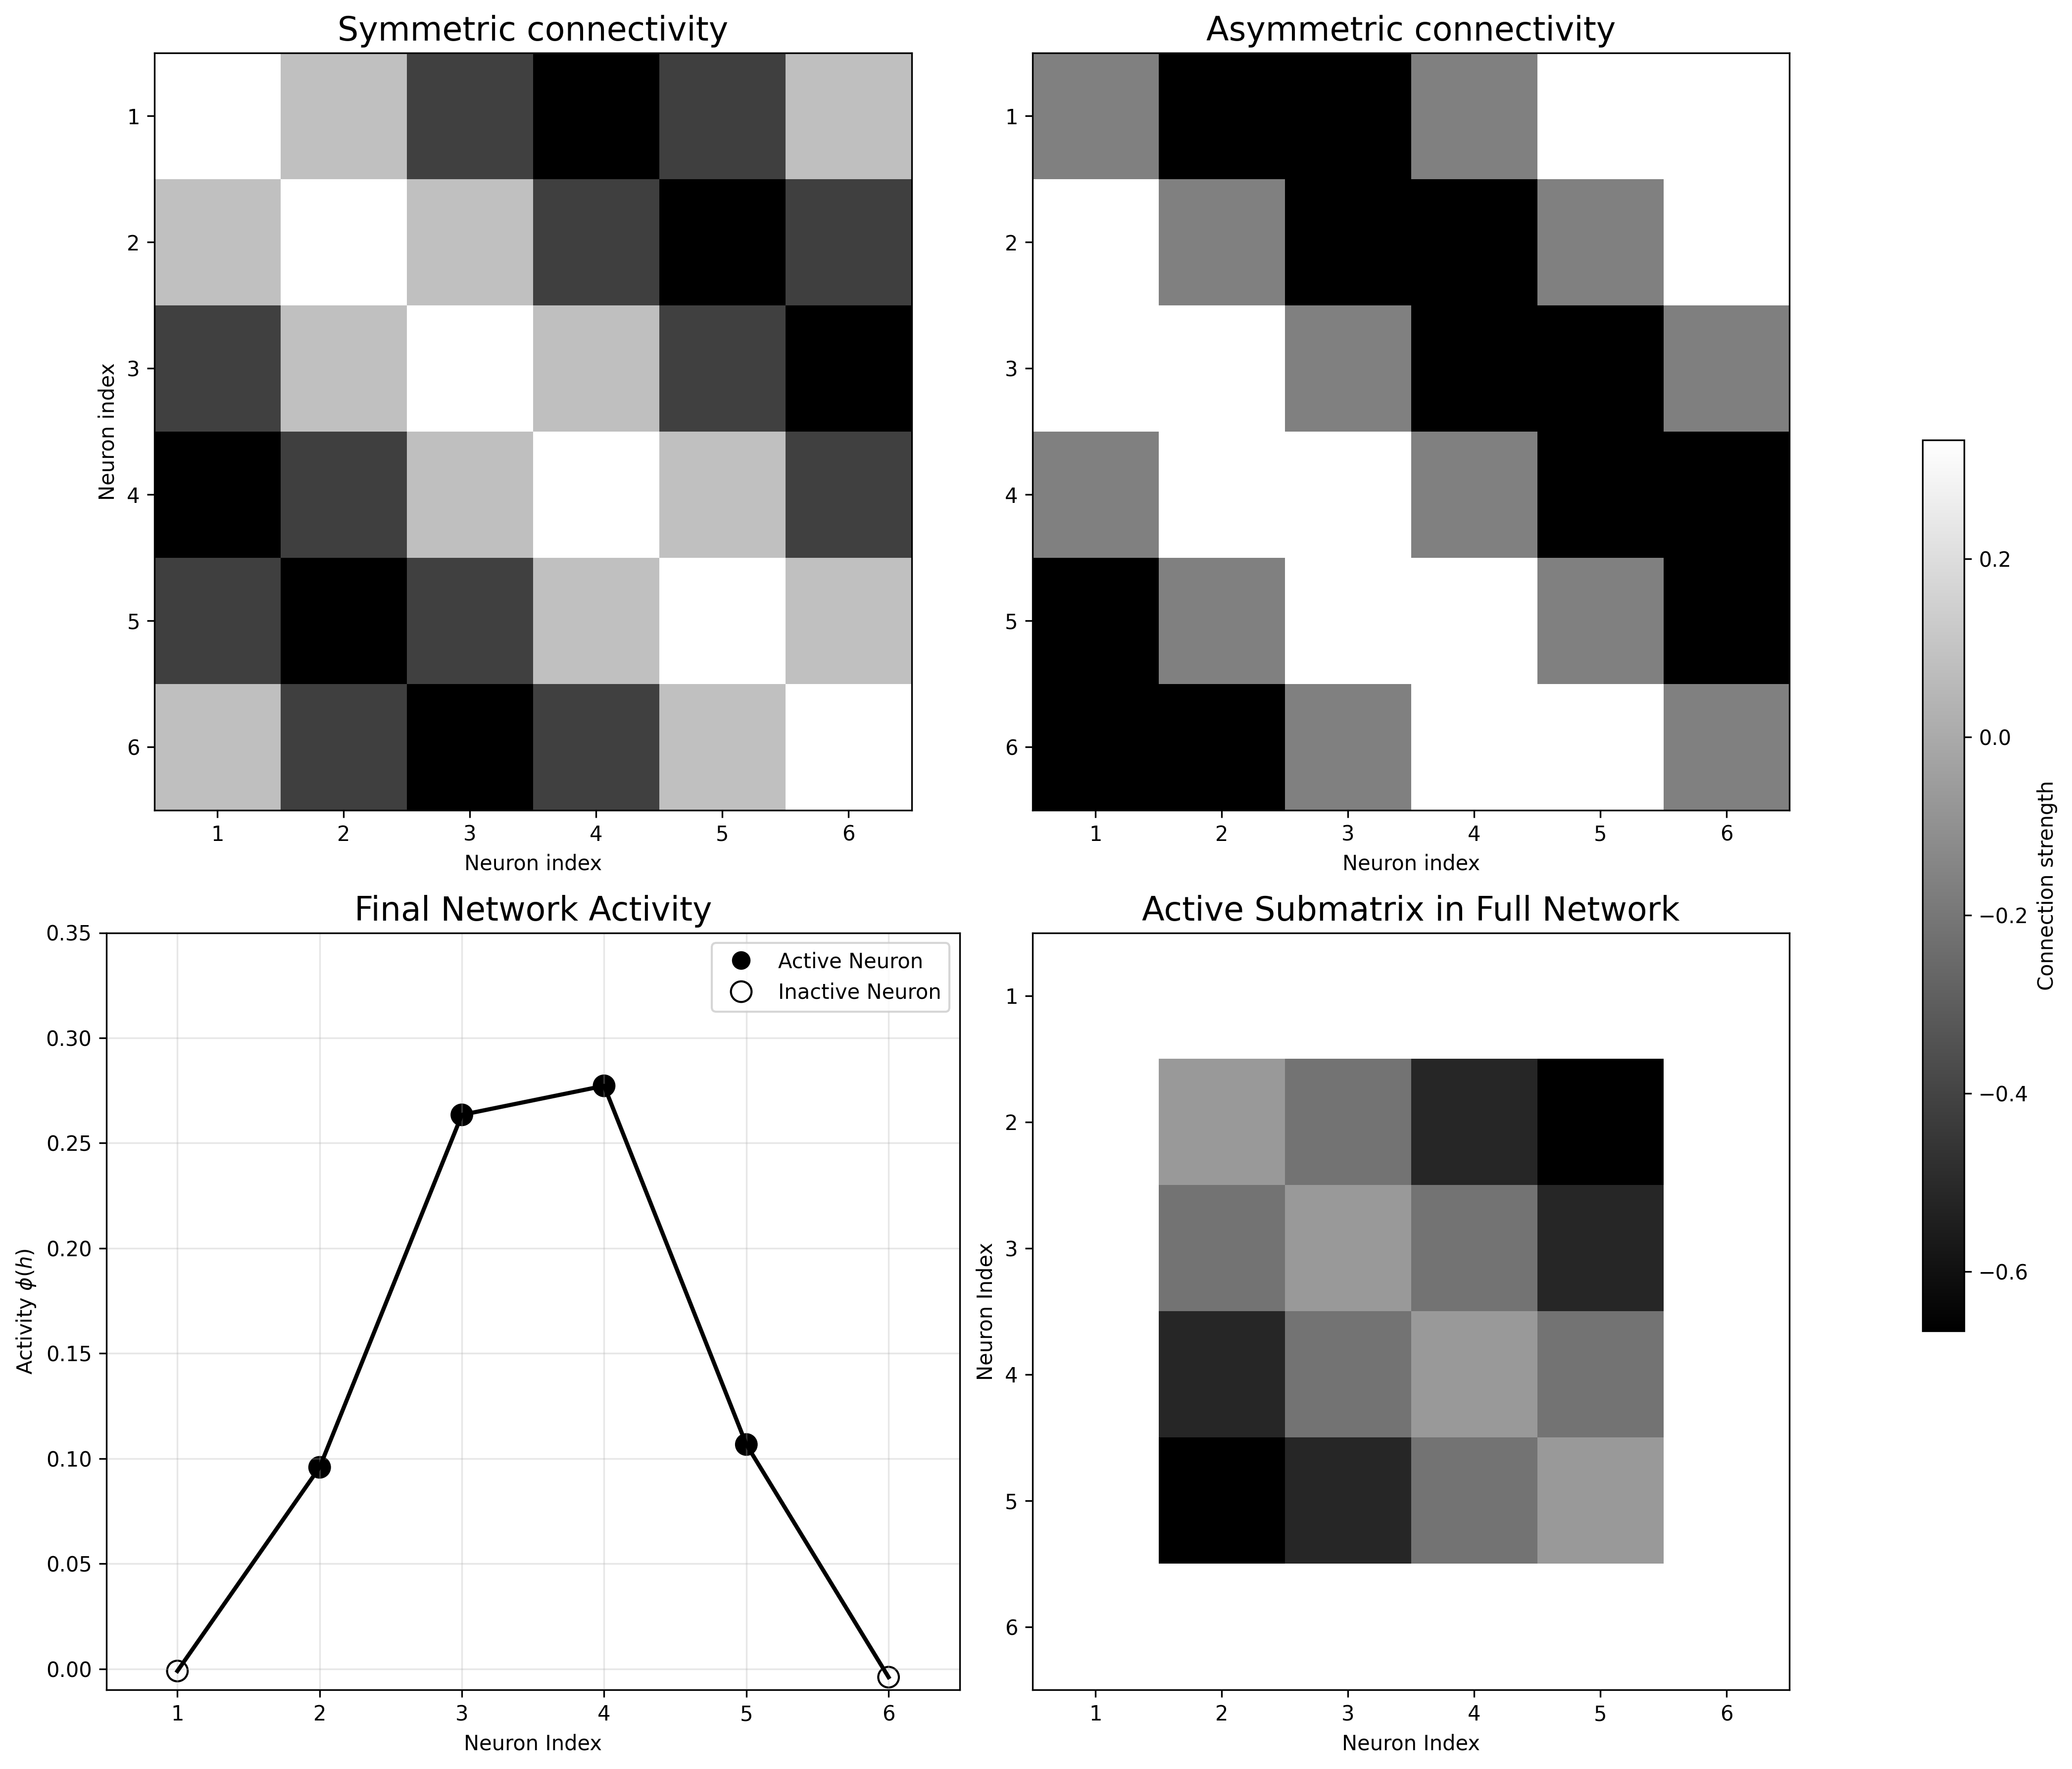
\includegraphics[width=0.8\textwidth]{connectivity_and_activity.png}
    \caption{Network structure and activity pattern of a 6-neuron ring attractor. \textbf{Top:} Symmetric weight matrix (left) implementing local excitation and global inhibition, and asymmetric weight matrix (right) for velocity integration. \textbf{Bottom:} Final network activity showing persistent bump with active neurons highlighted (left), and the corresponding submatrix of symmetric weights restricted to active neurons (right).}
    \label{fig:network_structure}
\end{figure}


\subsubsection*{PCA Analysis}

To analyze the structure of the network’s attractor dynamics, we applied Principal Component Analysis (PCA) to the population activity. We simulated a network of $N = 6$ neurons with parameters $J_I = -2.0$, $J_E = 4.0$, $v_{\text{in}} = 1.5$, and $c_{\text{ff}} = 1$, and recorded the full 6-dimensional neural activity across 1000 trials as the network encoded a continuously varying the orientation. 
We centered the activity data, computed the covariance matrix, and performed eigenvalue decomposition using \texttt{NumPy}. 



\section{Results}

\subsection{Stability Restults}

The authors analyze the stability of a small ring attractor network using a dynamical systems approach, showing that continuous representations of circular variables, like head direction, can be maintained with as few as four neurons. This is achieved by constructing a set of line attractors, each defined by a fixed subset of active neurons, and smoothly transitioning between them as the bump of activity shifts. These stitched-together line attractors form a continuous ring attractor manifold. The bump configuration is characterized by its amplitude \( a \), width \( w \), and orientation \( \psi \), and the dynamics reduce to three differential equations governing how these evolve over time. A fixed point, representing a stable bump, occurs when all three derivatives vanish. Crucially, the stability of these fixed points depends on whether perturbations in bump orientation decay (\( \lambda_\psi < 0 \)) or are neutrally stable (\( \lambda_\psi = 0 \)). The system achieves marginal stability (a continuous attractor) when the strength of local excitation \( J_E \) is tuned to an optimal value \( J_E^* \), satisfying:
\begin{equation}
\frac{1}{J_E^*} = \frac{1}{N} \sum_{k \in K_{\text{act}}} \sin^2(\theta_k - \psi^*)
\end{equation}

This ensures the curvature of the energy landscape is flattened along the ring, enabling drift-free persistent activity.

When the network is optimally tuned in this way, narrow and robust bumps form that do not drift in the absence of input, allowing the network to stably represent continuous angular variables. Perturbations orthogonal to the attractor manifold (i.e., changes in bump width or amplitude) are suppressed due to negative eigenvalues, while motion along the attractor (changes in \( \psi \)) is marginally stable. This tuning balances local excitation with global inhibition and ensures that the active submatrix of the recurrent connectivity has a zero leading eigenvalue, an indicator of line attractor dynamics. If \( J_E \) deviates from its optimal value, the bump either drifts toward discrete fixed points or becomes unstable. Thus, the network’s ability to maintain continuous attractor dynamics, and hence a faithful internal representation of variables like head direction, depends critically on fine-tuned parameters that place it near the boundary between stability and marginal stability.


% \begin{figure}[H]
% \centering
% % \includegraphics[width=0.7\textwidth]{figure1.png}
% \caption{[Figure caption explaining what is shown and key observations]}
% \label{fig:label1}
% \end{figure}



\subsection{PCA results}

\subsubsection*{Manual vs. \texttt{scikit-learn} PCA}

To validate the robustness of our PCA-based analysis, we compared the results of our manual implementation with those obtained using the \texttt{scikit-learn} library. 
Both methods produced identical eigenvalues and a cosine similarity of 1 between corresponding principal components (components beyond the third are nearly zero), confirming the correctness of our implementation (Figure~\ref{fig:...}). Minor visual differences observed in (Figure~\ref{fig:...}) are explained by the fact that PCA eigenvectors are only defined up to a sign; thus, some components appear flipped in direction, but still span the same subspace.




\subsubsection*{Low-Dimensional Ring Manifold}

Mapping the full neural state space onto the first three principal components reveals a pronounced \textbf{ring manifold} (Fig. ).
Colour–coding each point by its underlying head-direction angle exhibits a one-to-one, circular correspondence between behaviour and network state. 
The mild ripples along the third component are not energy bumps; they arise from finite-size bump-shape fluctuations and the sign indeterminacy of PCA axes. 
So the manifold remains energetically flat and effectively two–dimensional, indicating that the chosen $J_E$ is close to the optimal value $J_E^{\ast}$ that ensures continuity. 
In the following section, we examines how different initial conditions influence this ring.


\begin{figure}[H]
\centering
\begin{subfigure}{0.45\textwidth}
    \centering
    \caption*{\textbf{A}}
    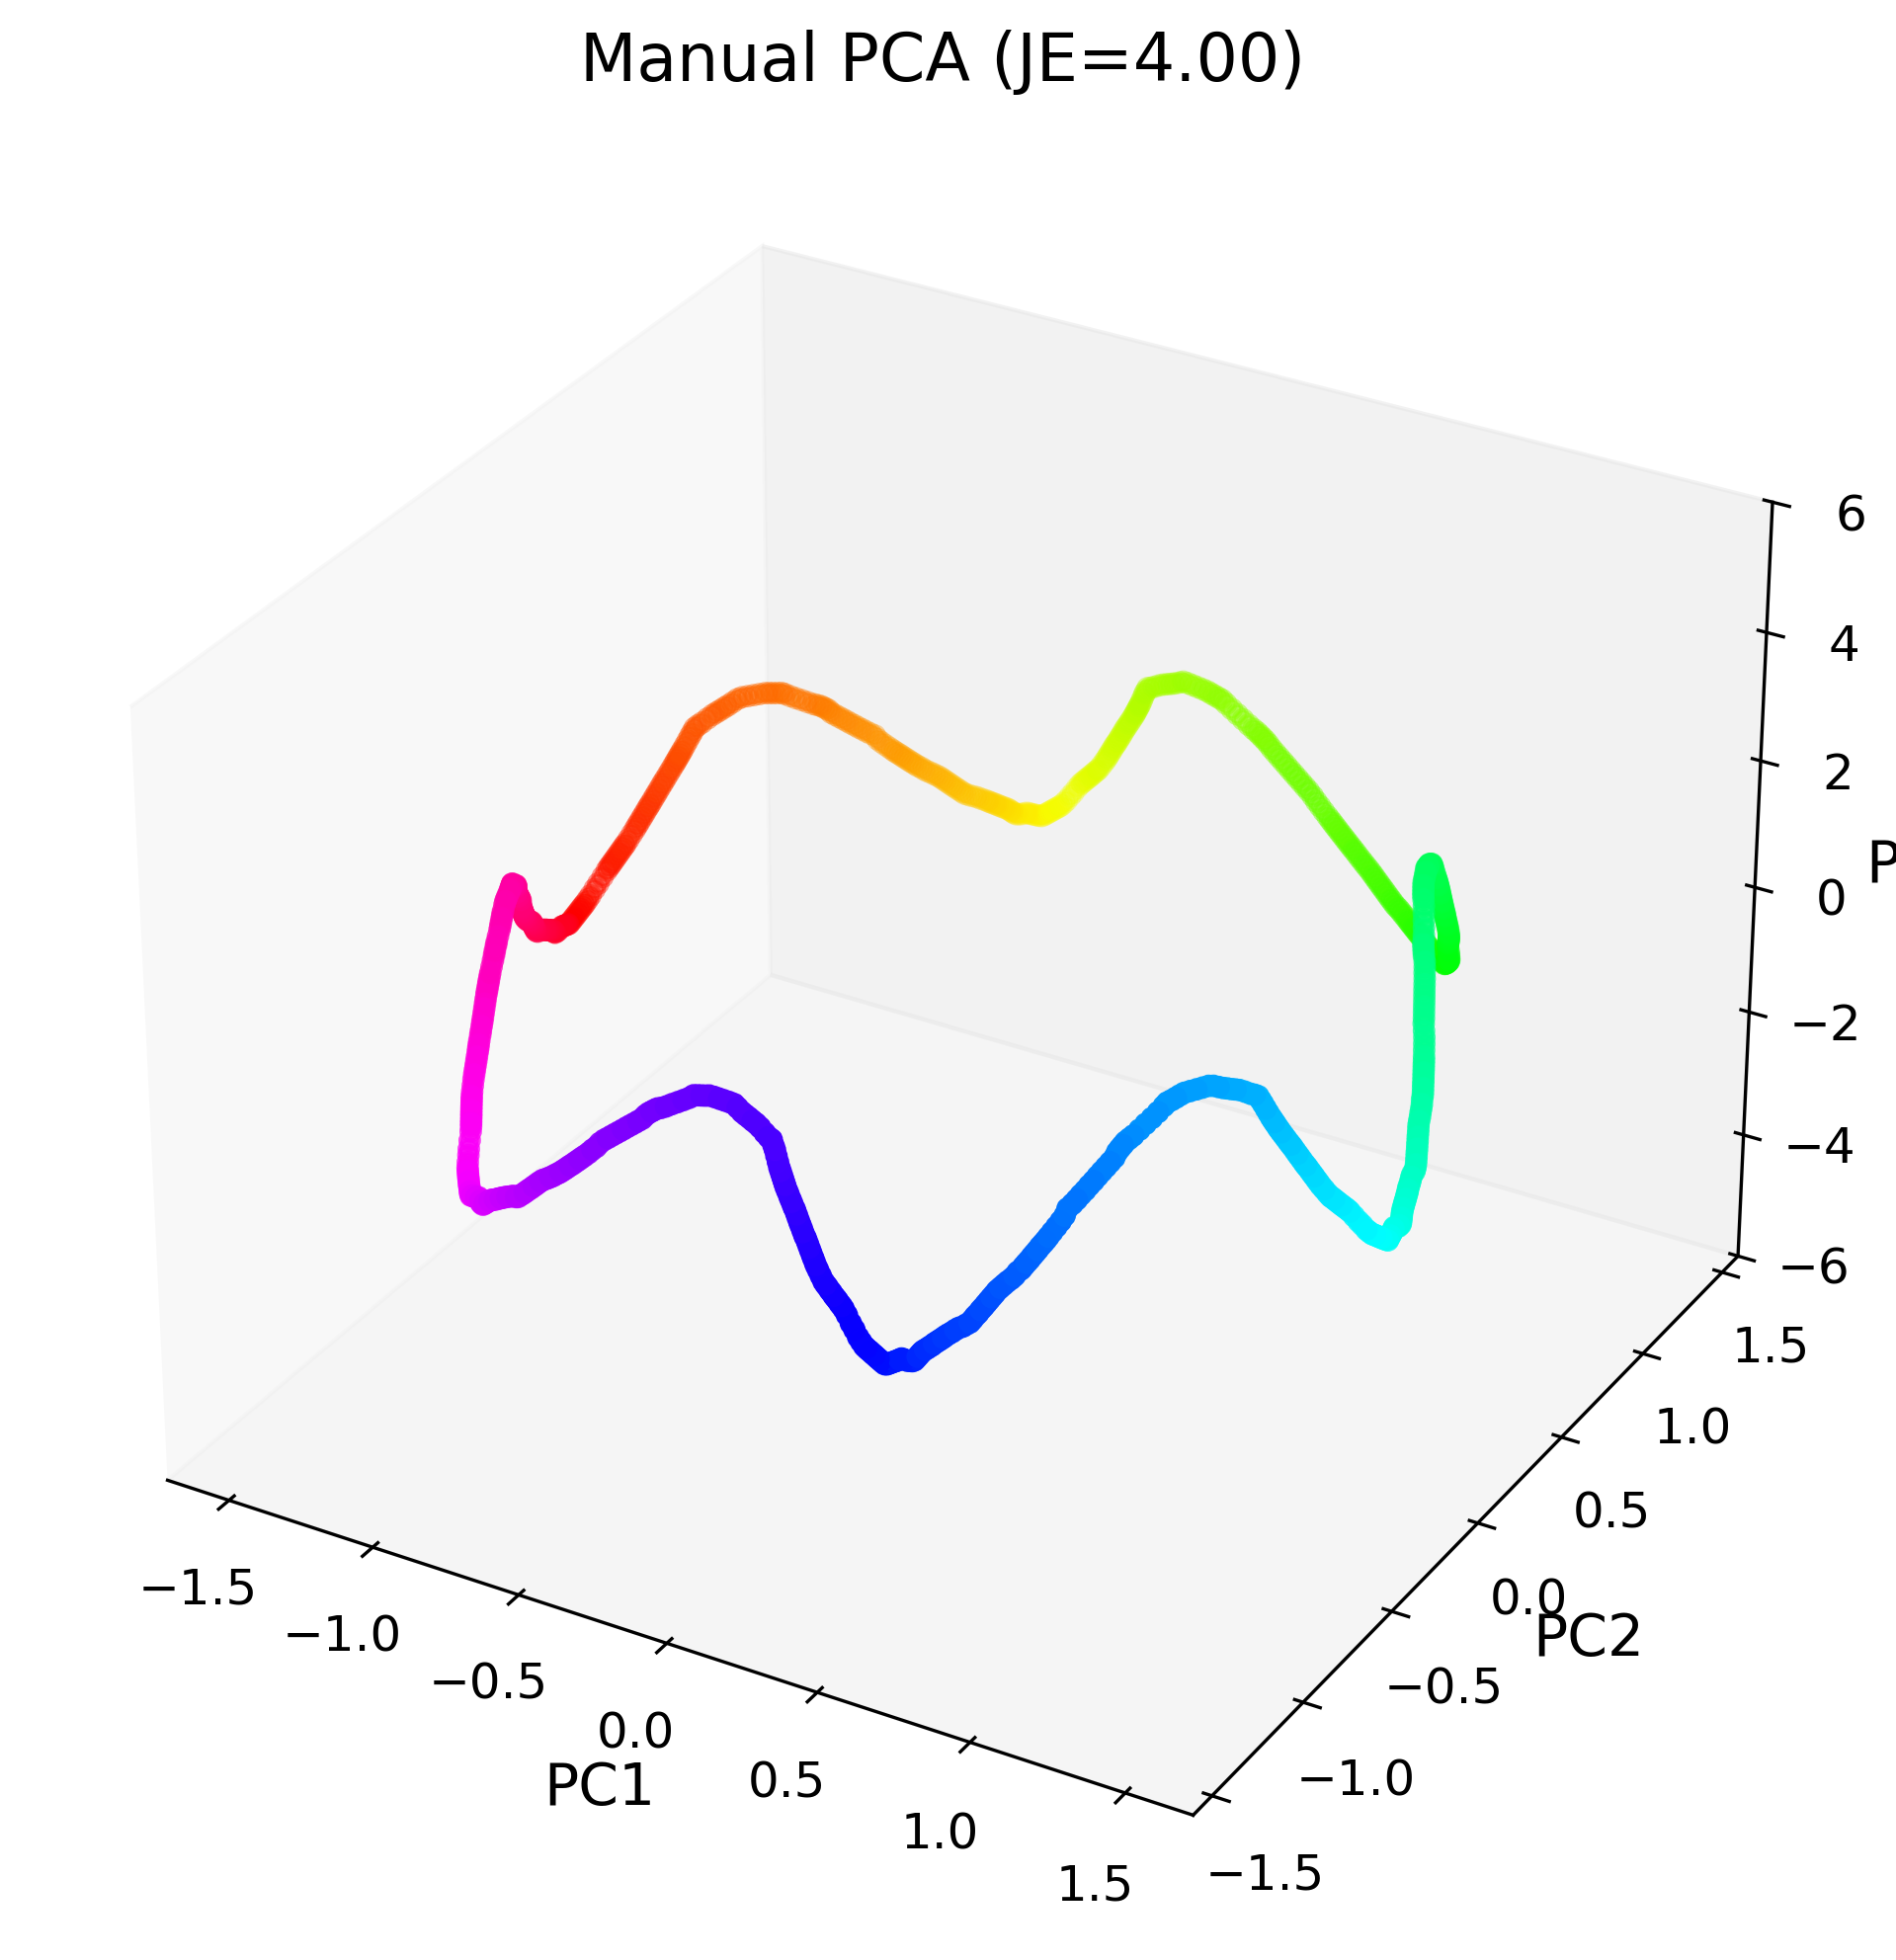
\includegraphics[width=\textwidth]{manual_pca.png}
    % \caption{Manual PCA implementation showing the first two principal components of neural activity. The circular pattern indicates a continuous ring attractor manifold where each point represents the final state of the network from different initial orientations.}
\end{subfigure}
\hfill
\begin{subfigure}{0.45\textwidth}
    \centering
    \caption*{\textbf{B}}
    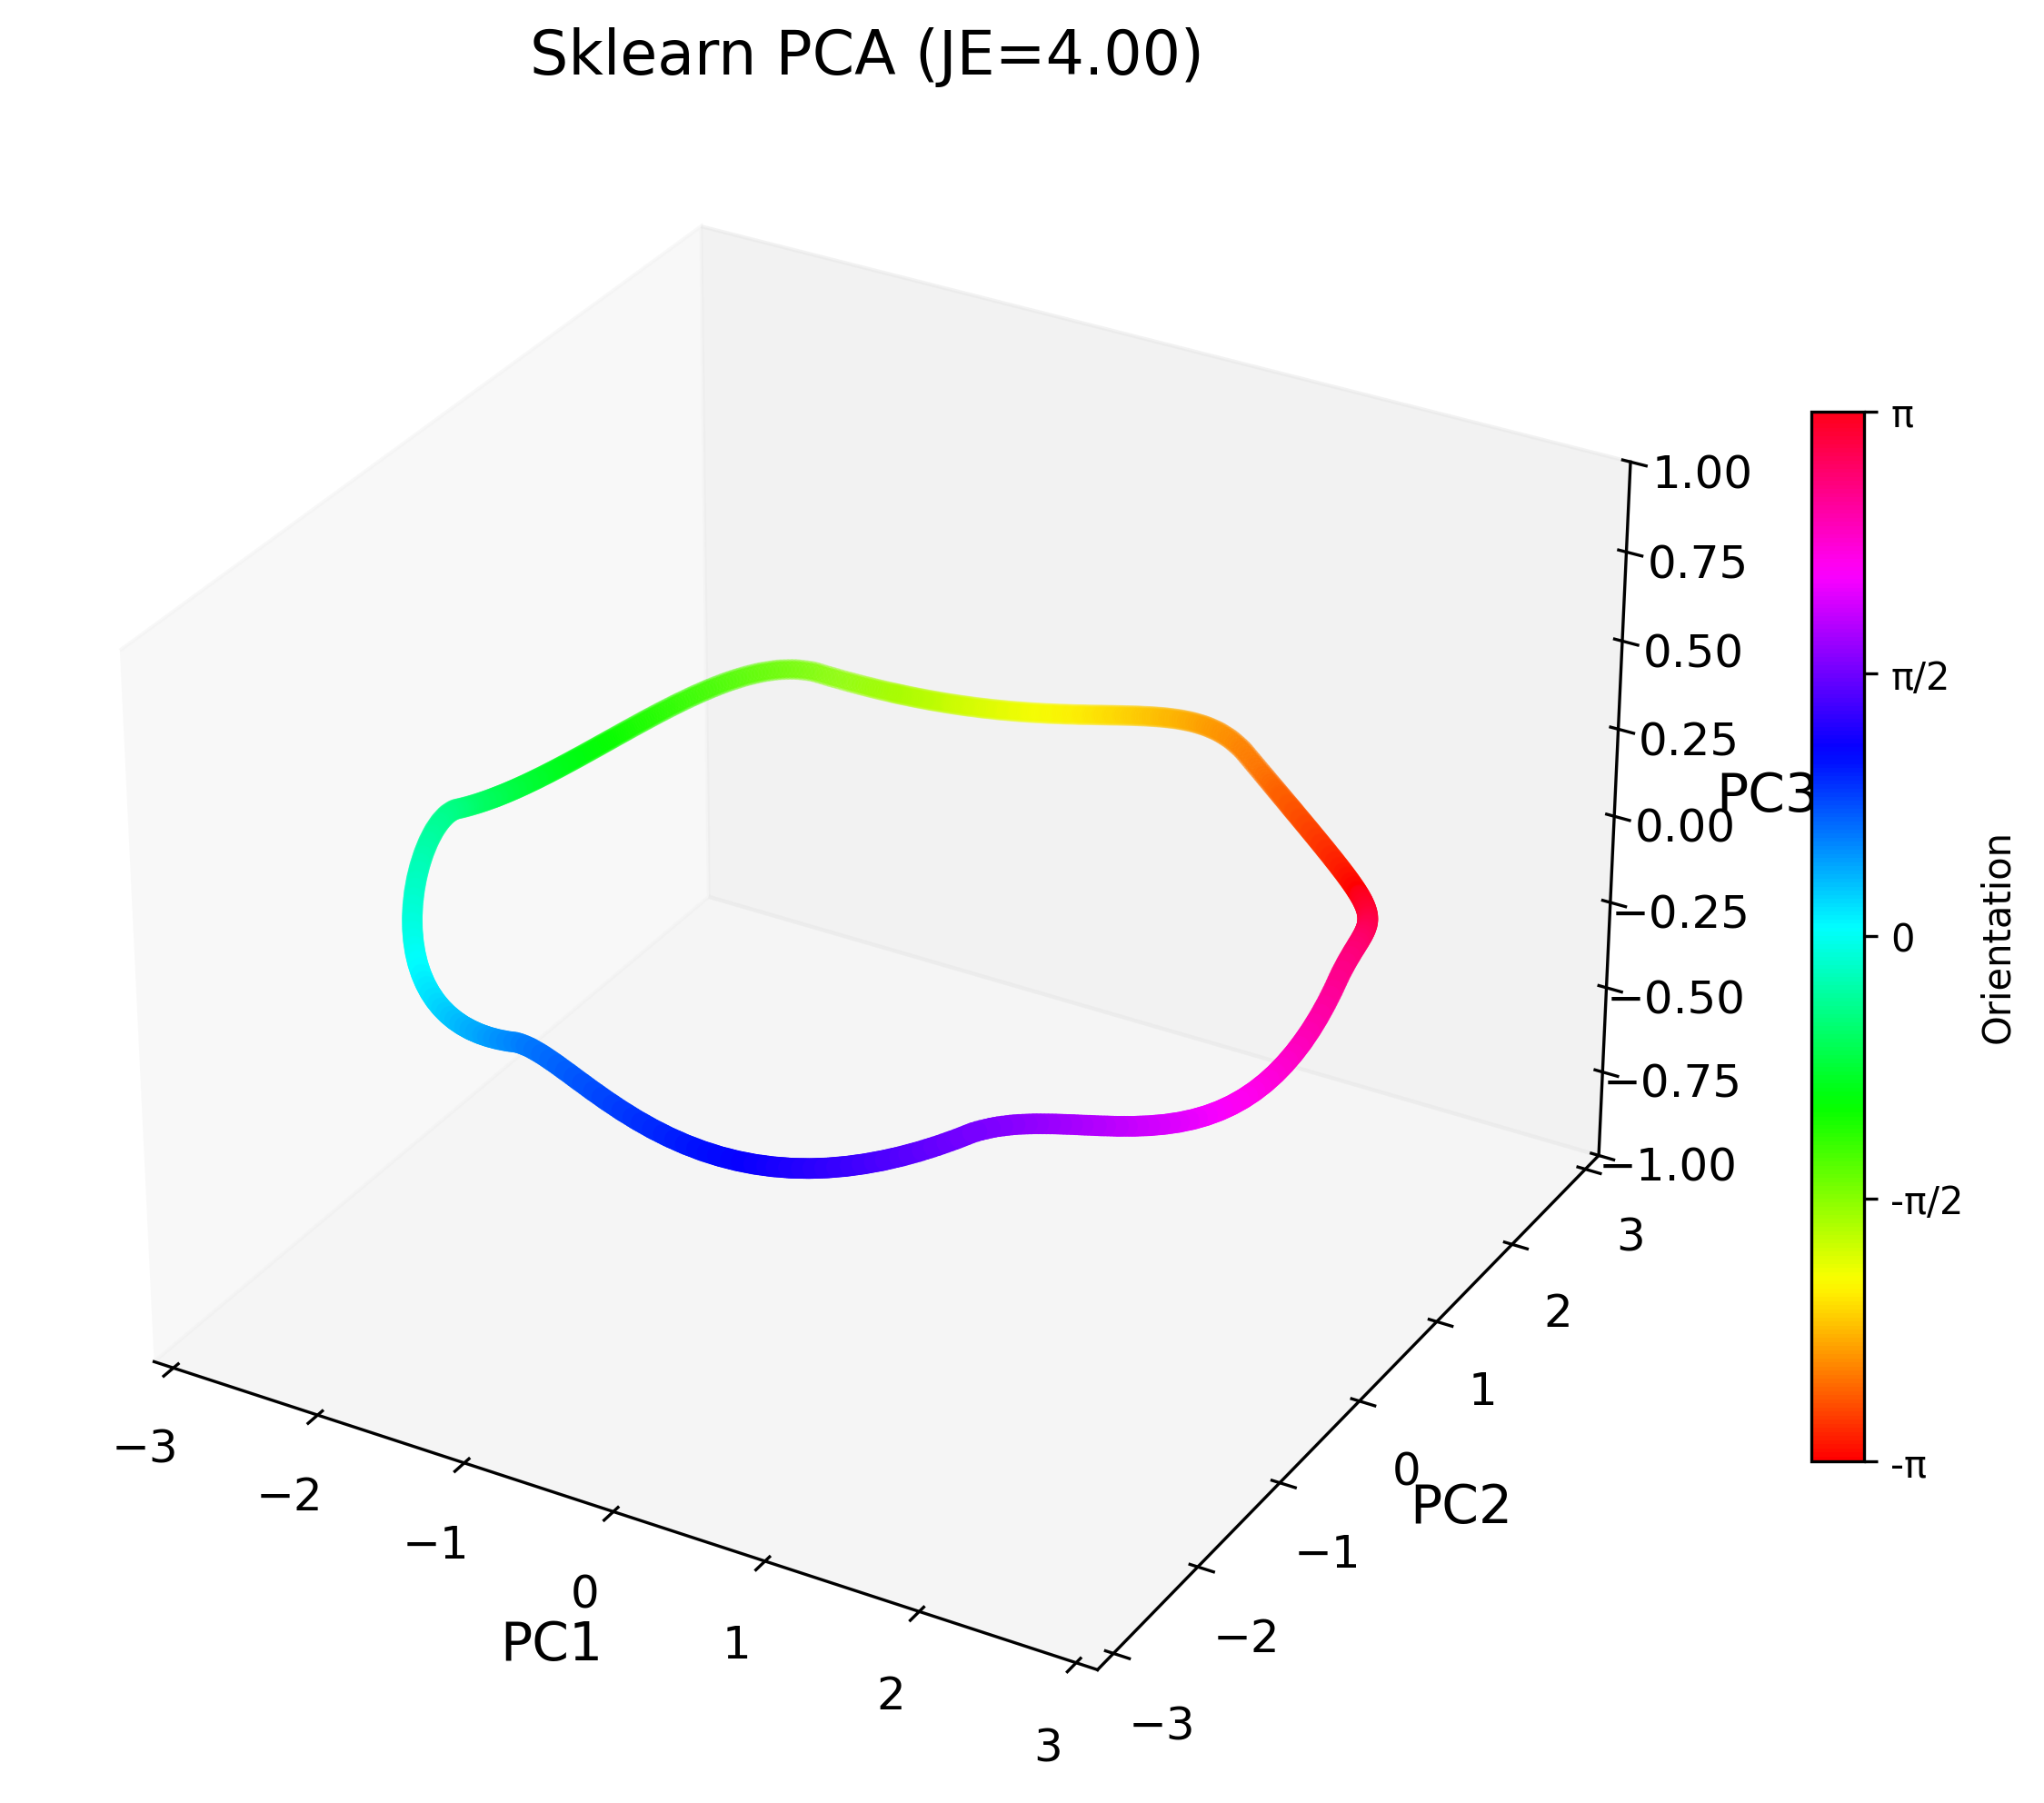
\includegraphics[width=\textwidth]{sklearn_pca.png}
    % \caption{Scikit-learn PCA implementation of the same data showing nearly identical results. The slight differences in orientation are due to sign ambiguity in eigenvector computation but preserve the same geometric structure.}
\end{subfigure}

\vspace{0.5cm}

\begin{subfigure}{0.45\textwidth}
    \centering
    \caption*{\textbf{C}}
    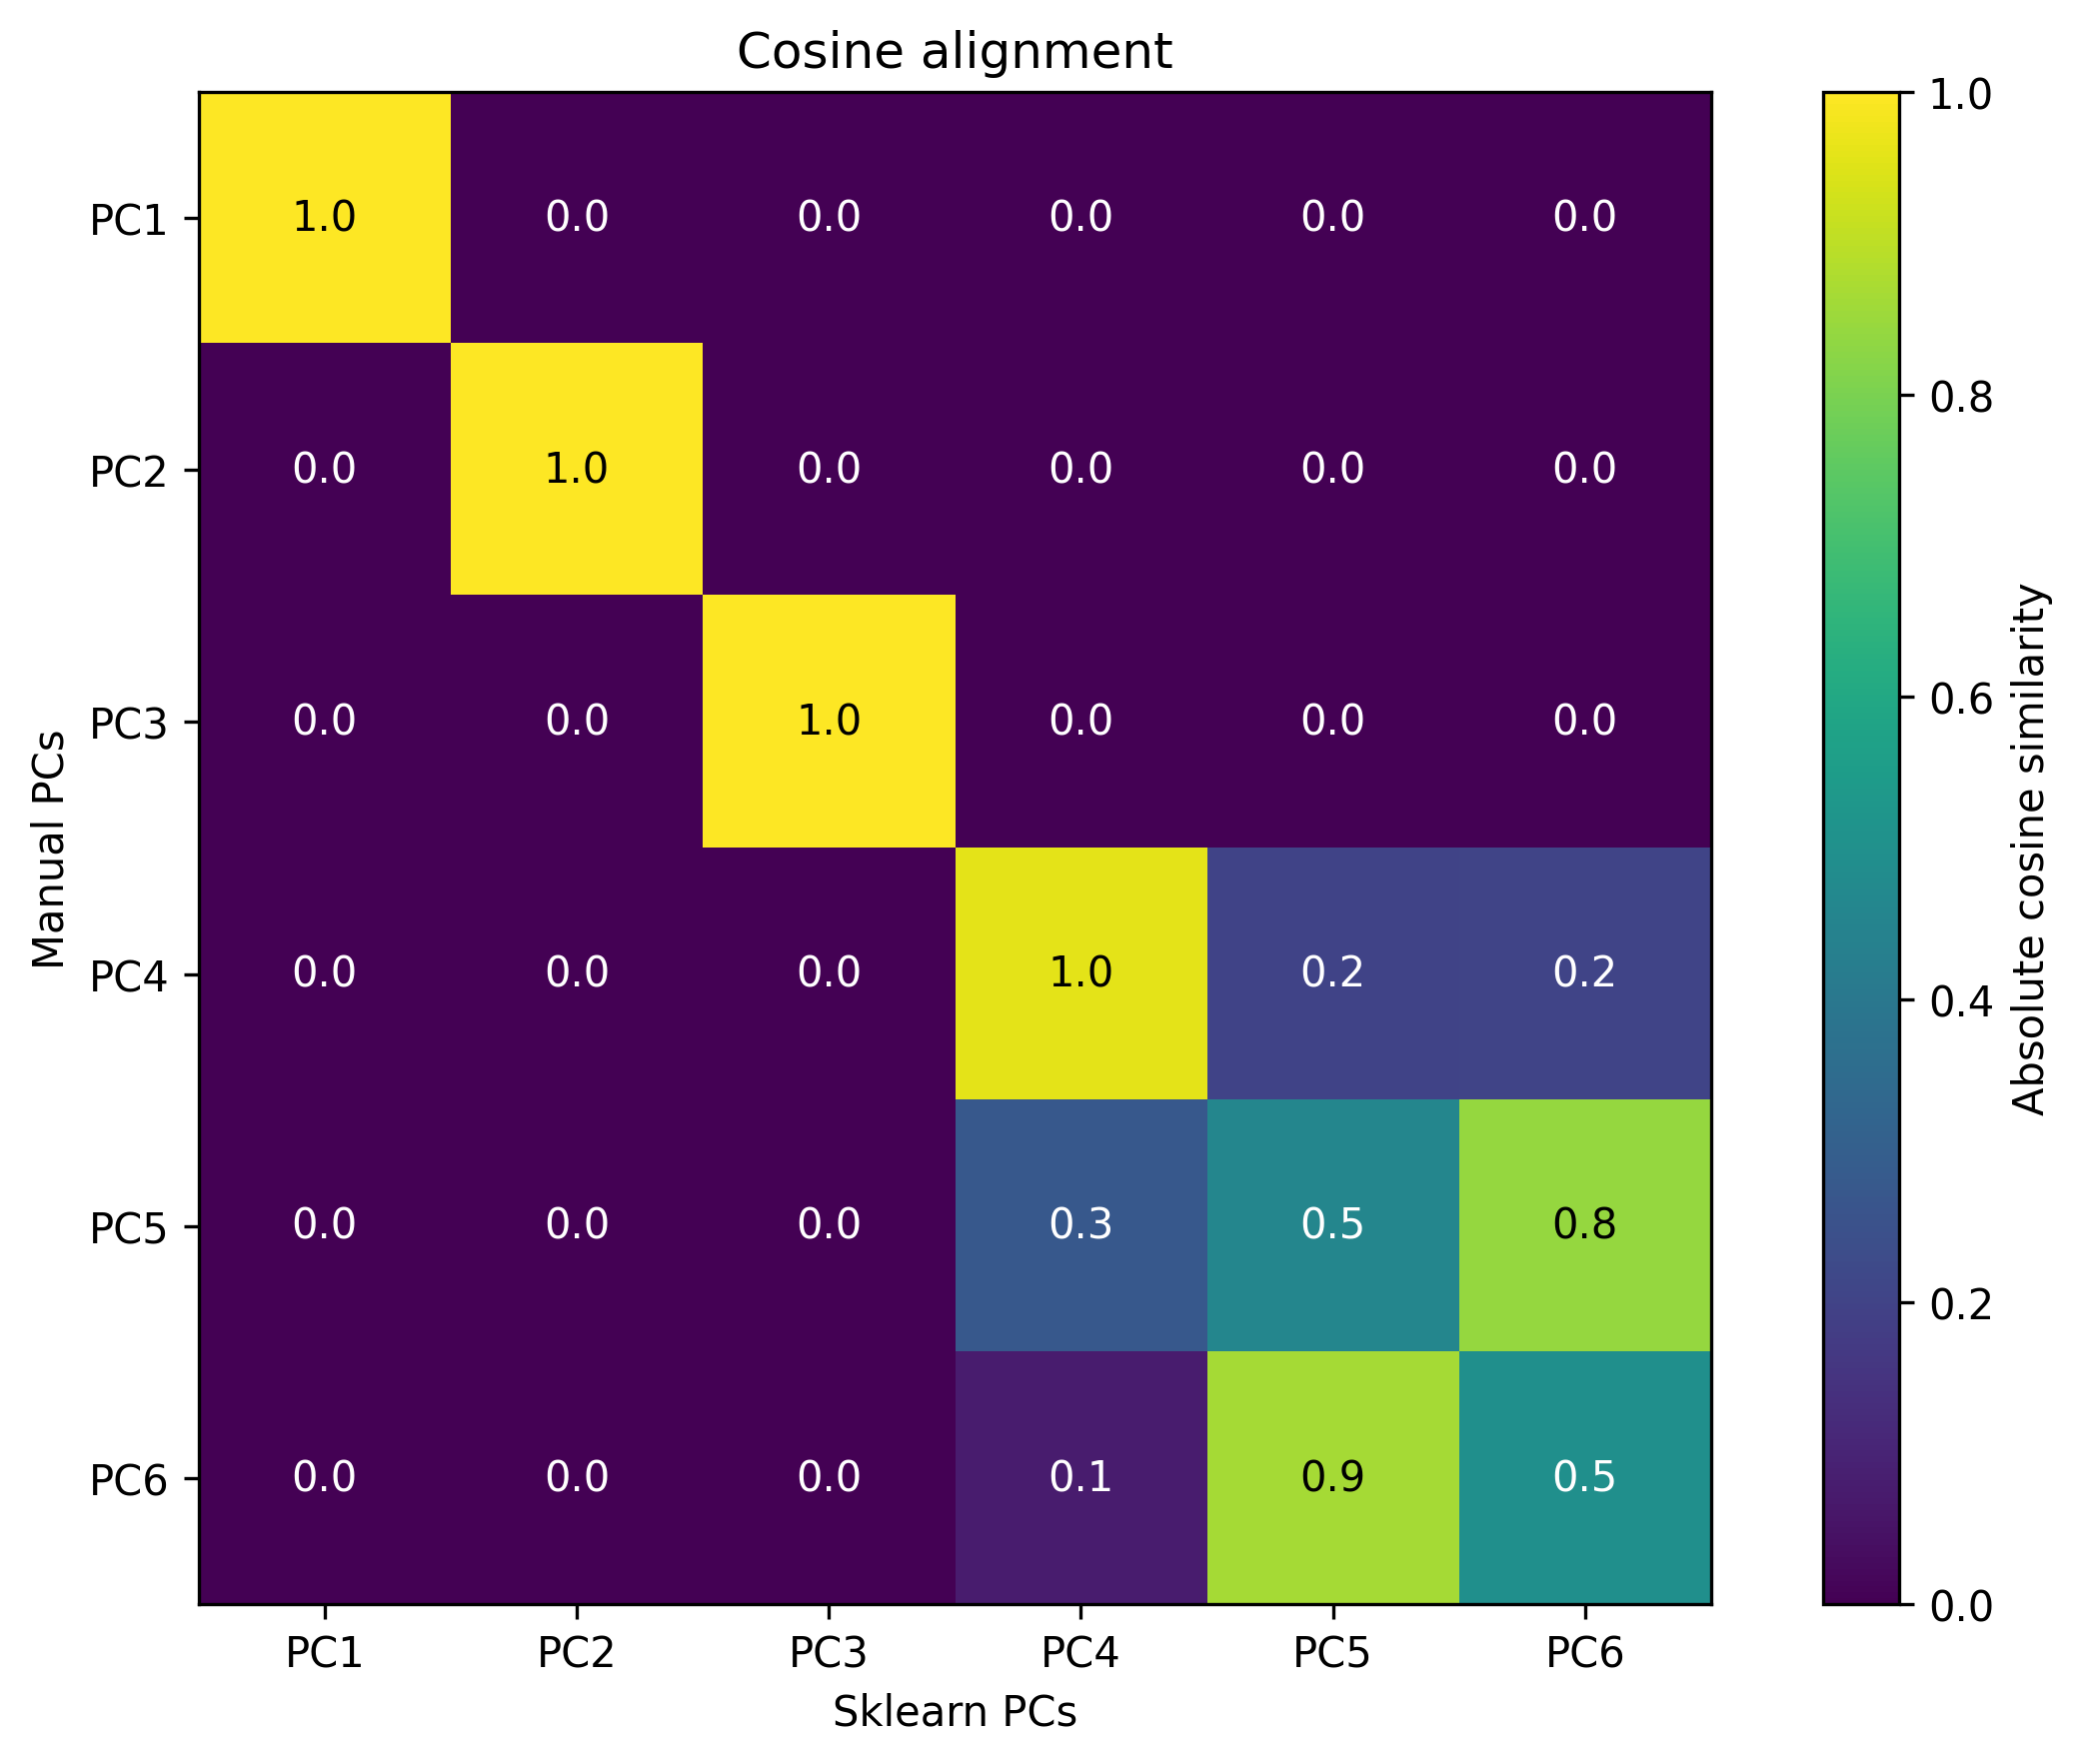
\includegraphics[width=\textwidth]{cosine_alignment.png}
    % \caption{Cosine similarity between manual and scikit-learn PCA components, showing perfect alignment (values of 1 or -1) for the first three components that capture over 99\% of variance. Negative values indicate flipped orientation of eigenvectors.}
\end{subfigure}
\hfill
\begin{subfigure}{0.45\textwidth}
    \centering
    \caption*{\textbf{D}}
    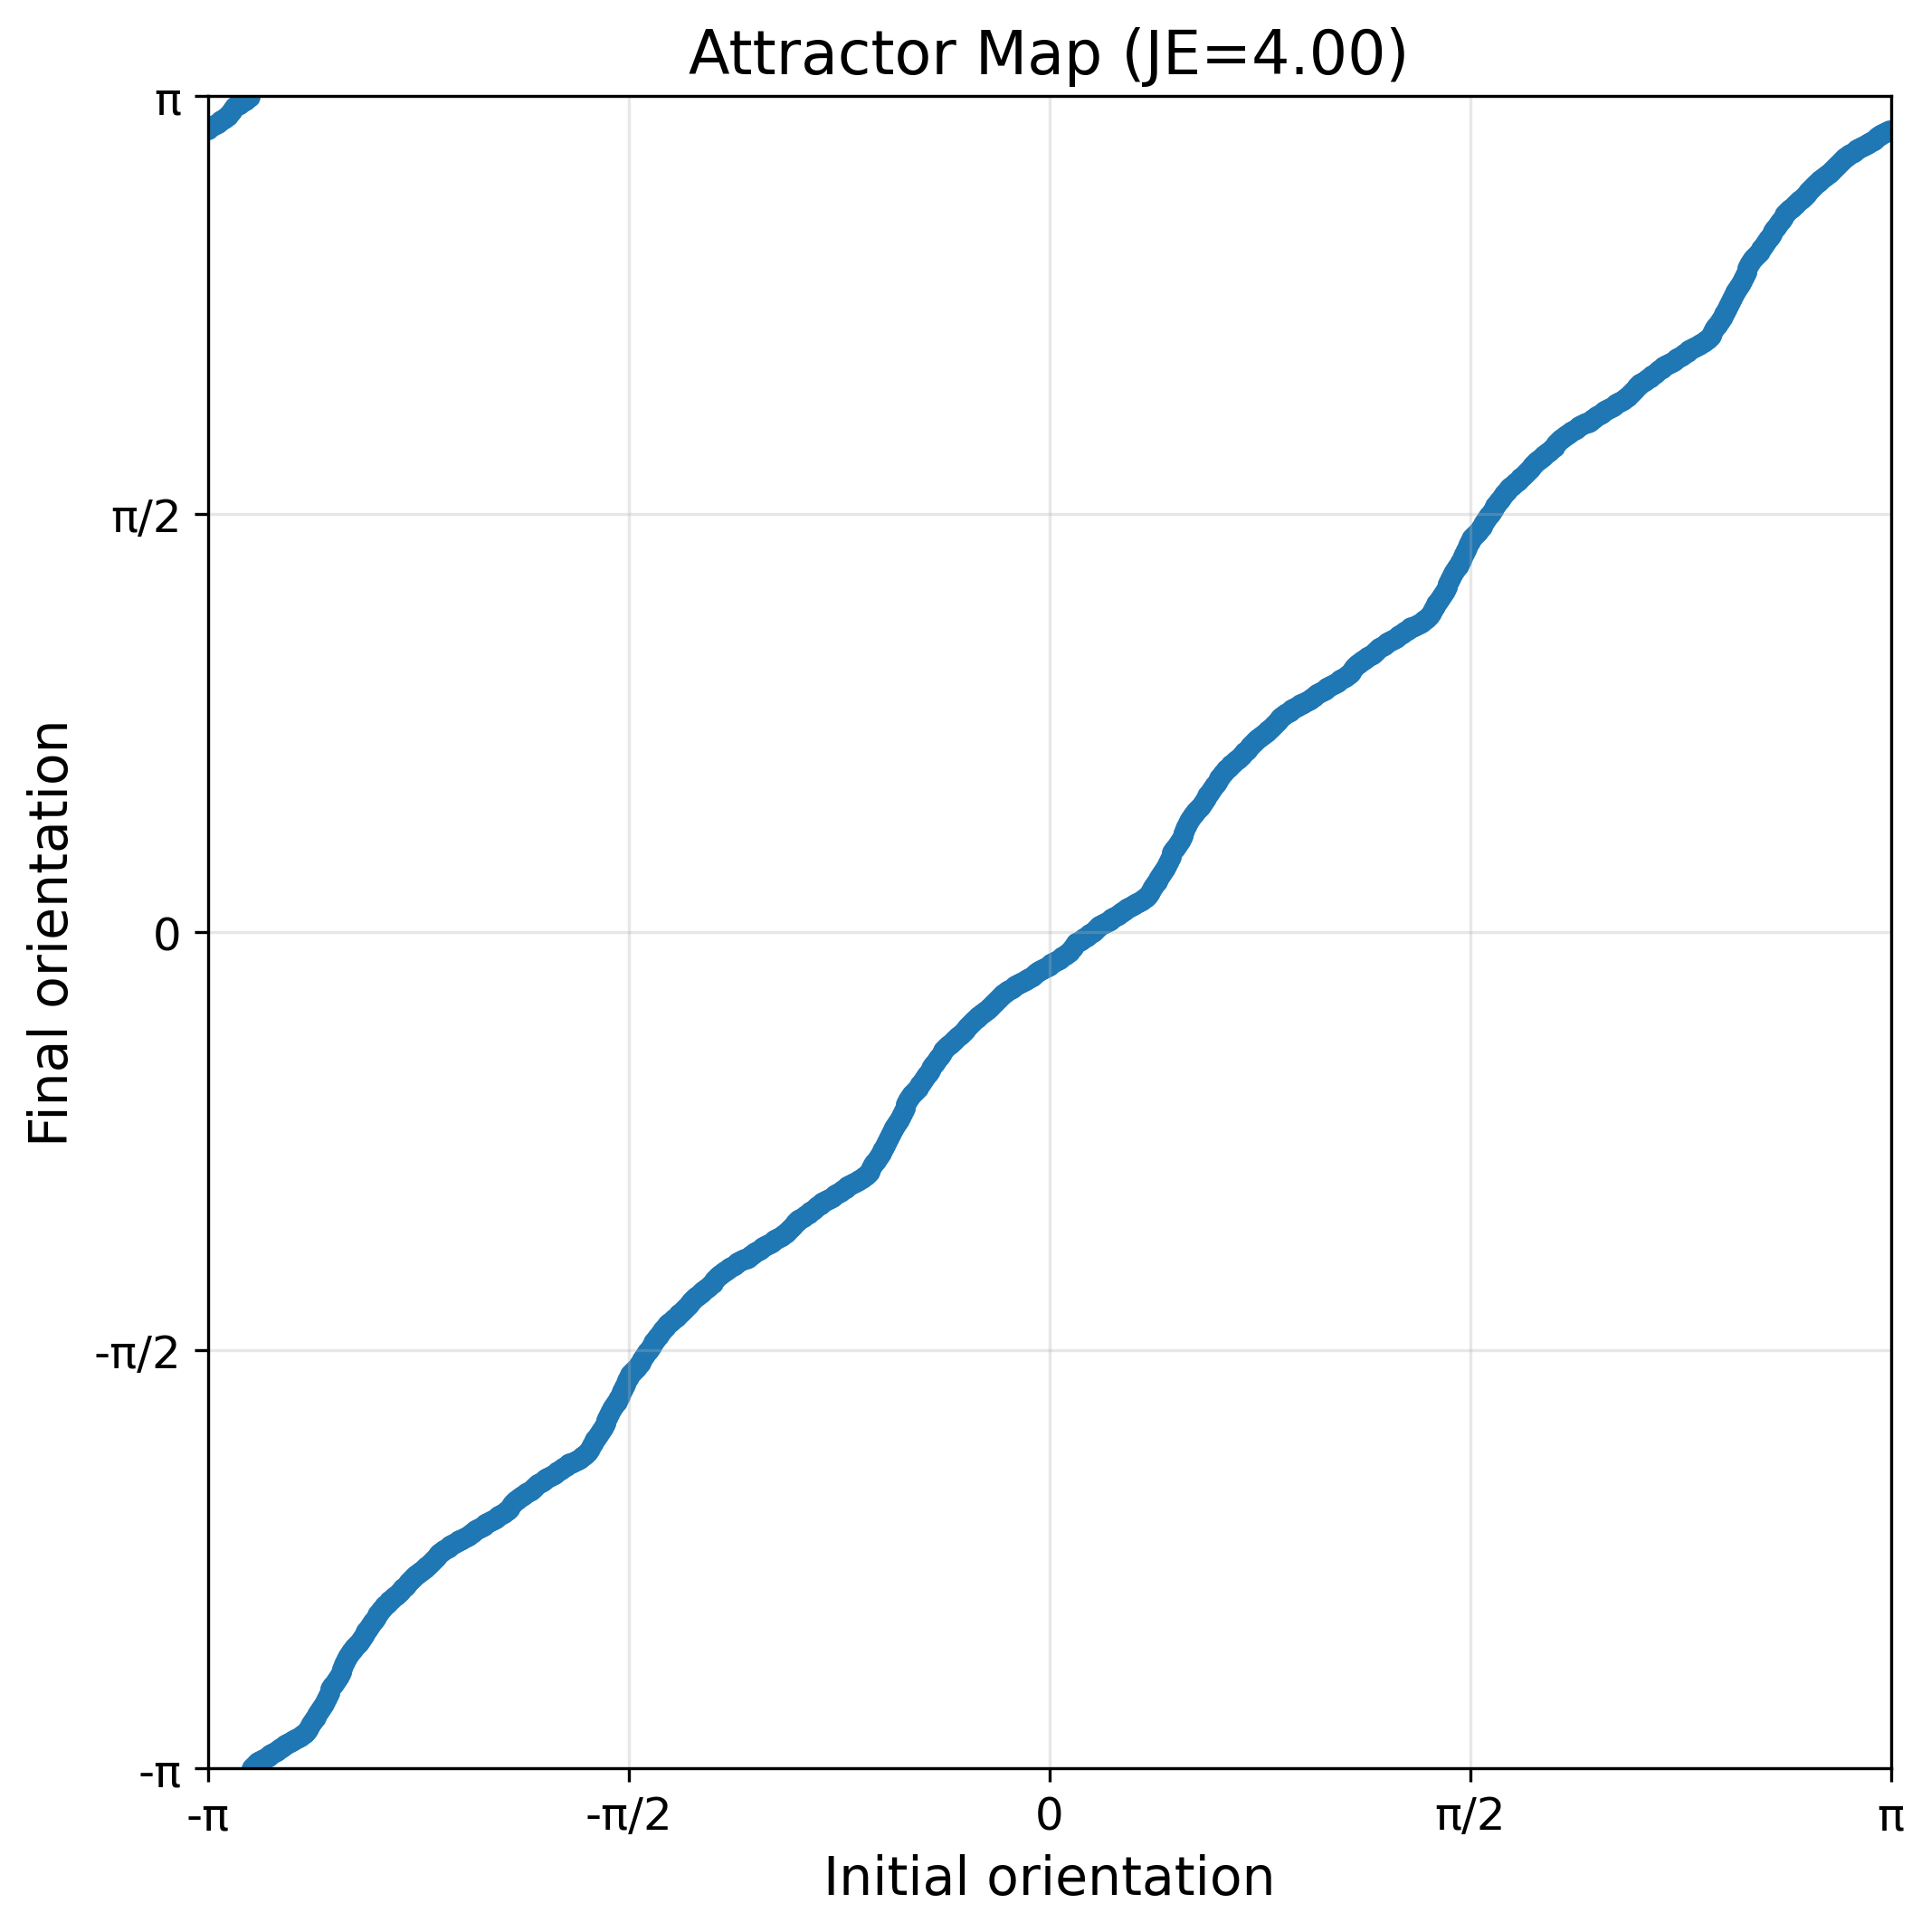
\includegraphics[width=\textwidth]{orientation_comparison.png}
    % \caption{Final vs. initial orientation in the network ($J_E = 4.0, J_I = -2.0$). The one-to-one relationship confirms that the network maintains a continuous representation of orientation with no preferred discrete states or drift.}
\end{subfigure}

\caption{PCA analysis of ring attractor network dynamics. (A,B) Both manual and scikit-learn PCA implementations reveal a circular manifold in the first two principal components, indicating a continuous ring attractor. (C) The cosine alignment between methods confirms implementation correctness. (D) The network maintains all orientations without discretizing, demonstrating true continuous attractor dynamics.}
\label{fig:pca_analysis}
\end{figure}


\subsection{Influence of Different Parameter Sets}

\subsubsection*{Different Values of \( J_E \) without Angular Velocity Input}


To investigate how network stability depends on synaptic tuning, we varied the local excitation strength \( J_E \) over the six values examined in Fig.~2 of Noorman et al.—namely, \( J_E \in \{12, 6, 4, 3, 2.4, 1.2\} \), while fixing the broad inhibition at \( J_I = -2 \) and the constant feedforward drive at \( c_{\text{ff}} = 1 \). These values span the range from weak to strong excitation relative to the analytically derived optimal values \( J_E^\ast \) for a ring attractor in a network with \( N = 6 \) neurons.

Fig N illustrates how the network dynamics qualitatively shift across this range. 
At the two extremes—strong excitation (\( J_E = 12 \)) and weak excitation (\( J_E = 1.2 \))—the bump of activity does \emph{not} collapse onto a finite set of stable orientations. 
Instead, the network fails to stabilize, exhibiting persistent or drifting dynamics that do not converge to attractor states. 
% These regimes lie outside the range of optimal tuning, where either excessive excitation or insufficient recurrent support prevents the formation of discrete or continuous attractors.

At intermediate values such as \( J_E = 6 \) and \( J_E = 3 \), the dynamics exhibit partial stabilization: although the raw activity may initially form a broad cloud, it eventually contracts onto a small number of stable head-direction angles, consistent with discrete point attractors in PCA space. 
This indicates that the network relaxes into isolated fixed points rather than maintaining a continuous representation.

Interestingly, two finely tuned values, \( J_E = 4 \) and \( J_E = 2.4 \), yield qualitatively different behavior. 
In these cases, the population activity traces out a near-continuous ring in the first two principal components, with characteristic six-fold symmetry arising from the network size \( N = 6 \). 
Minor gaps at specific orientations are expected from finite-size sampling, but the attractor manifold remains effectively continuous. 
These two values correspond to analytically identified optimal excitation strengths that flatten the energy landscape along the angular dimension, enabling the network to support a marginally stable bump across the full ring.

Together, these results reveal a phase-like transition in the attractor structure: only near the optimal values of \( J_E \) does the system maintain a continuous head-direction code. 
Away from these values, the network either relaxes into discrete attractor states or fails to stabilize altogether, underscoring the importance of synaptic tuning for supporting robust ring attractor dynamics in small networks.

\begin{figure}[H]
\centering
\begin{subfigure}{\textwidth}
    \centering
    \caption*{\textbf{A}}
    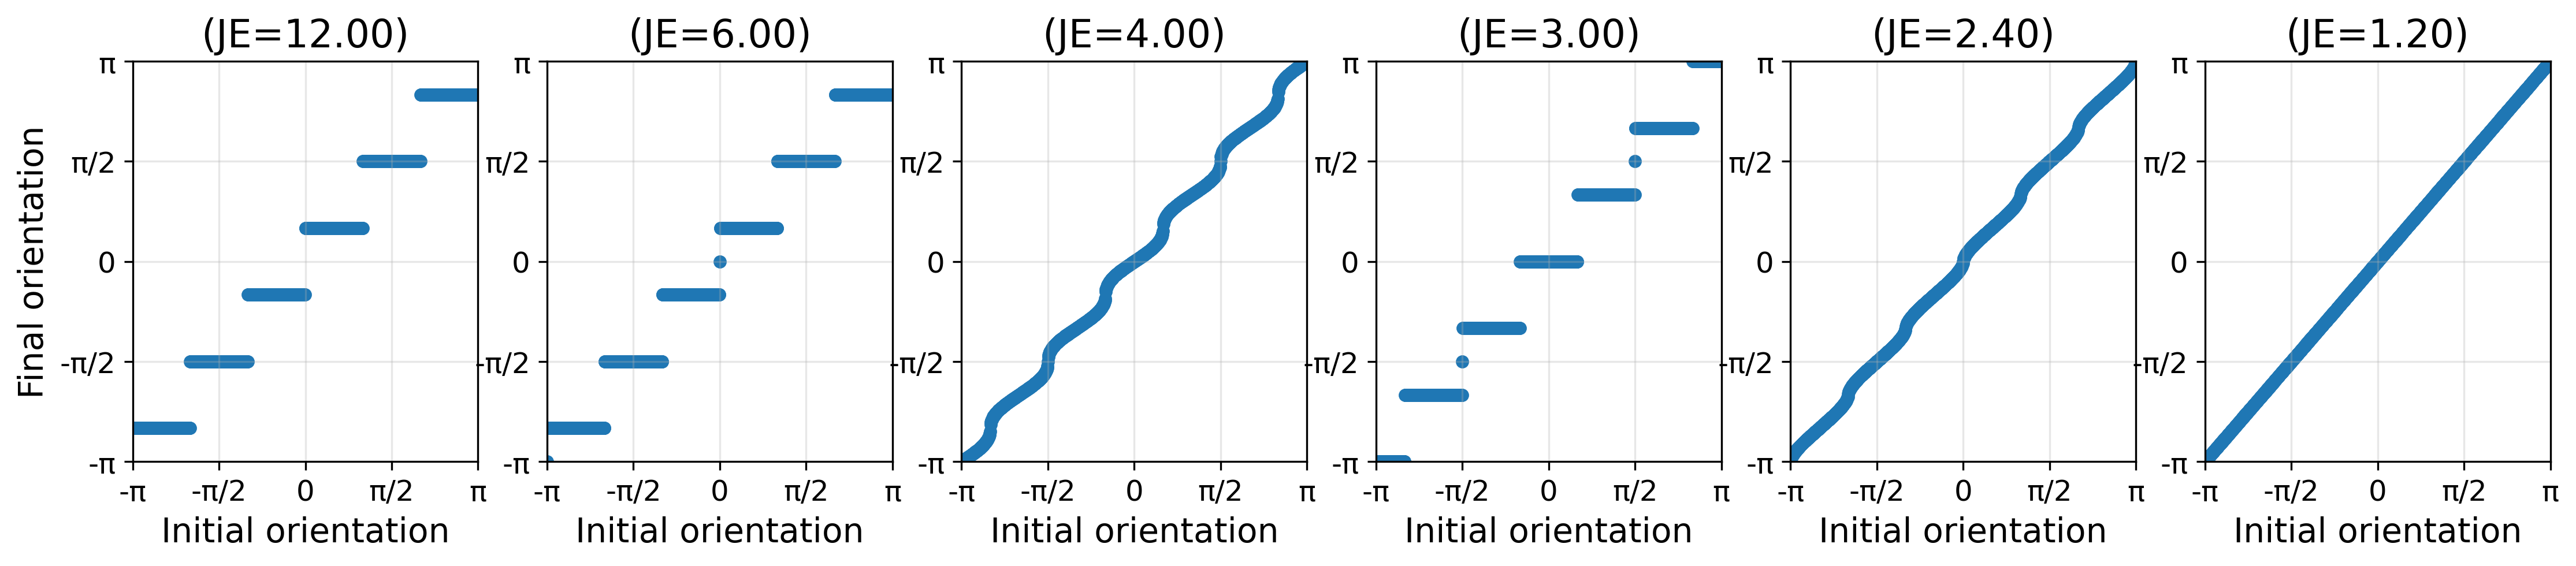
\includegraphics[width=\textwidth]{orientation_comparison_without_v.png}
\end{subfigure}

\vspace{0.1cm}

\begin{subfigure}{\textwidth}
    \centering
    \caption*{\textbf{B}}
    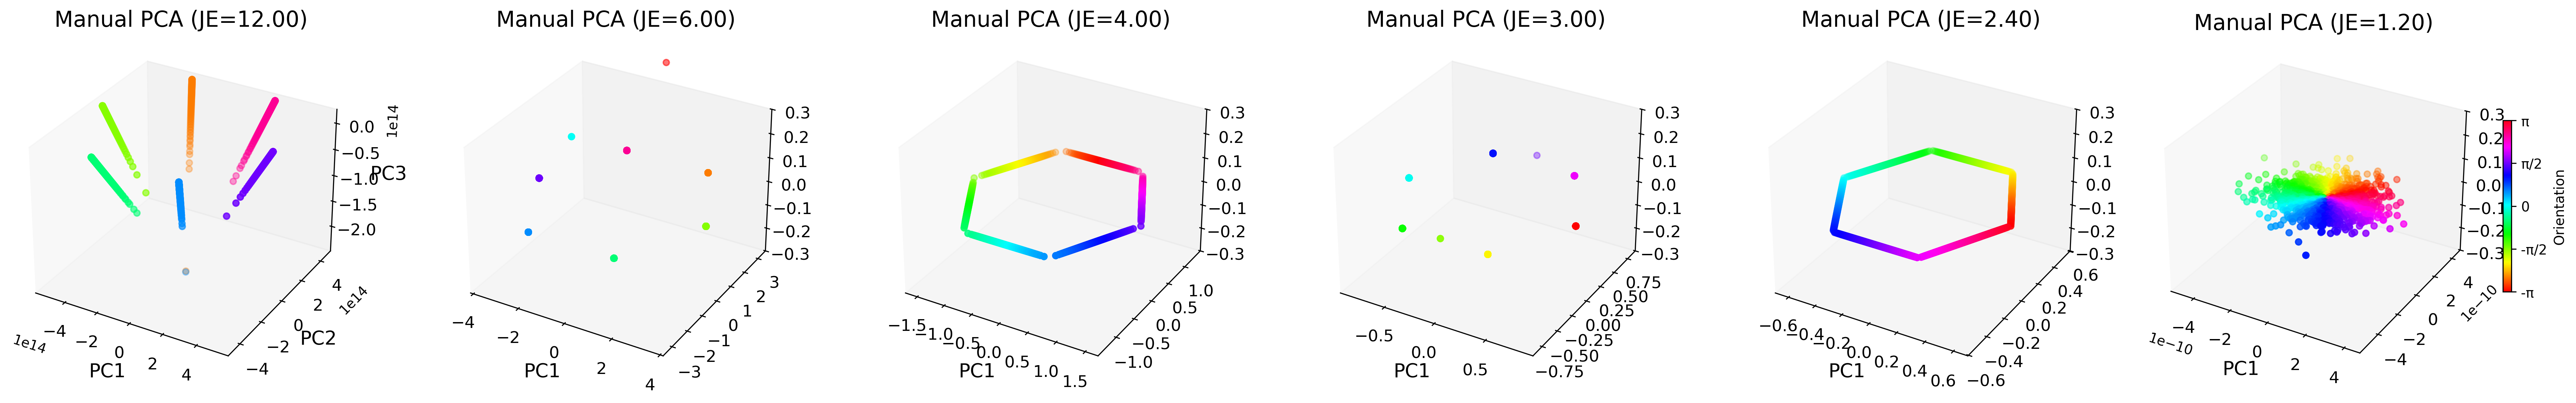
\includegraphics[width=\textwidth]{manual_pca_without_v.png}
\end{subfigure}

\caption{Effect of excitation strength \( J_E \) on ring attractor dynamics. (A) Final vs. initial orientation for six different values of \( J_E \). Perfect diagonal relationships indicate continuous attractor behavior, while discrete clusters points indicate breakdown of the ring manifold. 
(B) Corresponding 3D PCA representations showing the attractor manifold structure. Smooth ring-like trajectories emerge at optimal \( J_E \) values (4.0 and 2.4), while other parameter settings produce either discrete point attractors or unstable dynamics.}
\label{fig:je_parameter_sweep}
\end{figure}



\subsubsection*{Different Values of \( J_E \) with Angular Velocity Input}
Here we varied the local excitation strength \( J_E \) while applying a constant angular velocity input \( v_{\text{in}} = 1.5 \). 
This input biases the bump motion, allowing us to explore how the network dynamics respond to both synaptic tuning and external drive.


\section{Discussion}

[Interpret your results and relate them to your research question. Compare your findings with existing literature. Address limitations of your approach and suggest potential improvements or future directions.]

\section*{Conclusion}

The PCA revealed the geometry of the attractor manifold: when the network supports a continuous ring attractor, the final states trace a smooth circular trajectory in principal component space; in contrast, discretized networks exhibit distinct clusters corresponding to stable point attractors. 


[Summarize your key findings and their implications. Emphasize the significance of your work and how it contributes to the field.]

Key findings include:
\begin{itemize}
\item [Finding 1]
\item [Finding 2]
\item [Finding 3]
\end{itemize}

[Final concluding statement]

\section*{References}

[Include your references here or use a bibliography system like BibTeX]

\end{document}
